% % When working with unit operations that involve matrix operations dealing with vectors of different dimensions, the order in which we apply the chain rule matters .
% When computing a gradient using AD, we can encounter vector-Jacobian products (VJPs) or Jacobian-vector products (JVPs).
% % As their name indicates, the difference between them is that the quantity we are interested in is described by the product of a Jacobian times a vector on the left side (VJP) or the right (JVP).
% % Furthermore, both forward and reverse AD can be thought of as a way of computing derivatives associated with JVPs (see Equation \eqref{eq:directional-derivative}) and VJPs, respectively. 
% For each intermediate function $h: \R^{d_1} \mapsto \R^{d_2}$ that is evaluated when executing a given program, AD will perform the JVP operation $\dot x \mapsto Dh (x) \cdot \dot x$ in forward mode and the VJP operation $\bar y \mapsto \bar y^T \cdot Dh (x)$ (VJP) in reverse mode.
% Equivalently, forward AD map directional derivatives between tangent spaces, while reverse AD map vectors from co-tangent (or normal) spaces \cite{Griewank:2008kh}. 

Forward and reverse AD are based in the sequential evaluation of JVPs and VJPs, respectively. 
Let us consider for example the case of a loss function $L : \mathbb R^p \mapsto \mathbb R$ taking a total of $p$ arguments as inputs that is computed using the evaluation procedure $L(\theta) = \ell \circ g_{k} \circ \ldots \circ g_2 \circ g_1(\theta)$, with $\ell : \mathbb R^{d_k} \mapsto \mathbb R$ the final evaluation of the loss function after we apply in order a sequence of intermediate functions $g_i : \mathbb R^{d_{i-1}} \mapsto \mathbb R^{d_i}$, where we define $d_0 = p$ for simplicity. 
If we perturb the parameter $\theta \rightarrow \theta + \delta \theta$, this will produce a perturbation $L (\theta) \rightarrow L(\theta) + \delta L$ in the loss function that can be computed at first order in $\delta \theta$ using the chain rule as: 
\begin{equation}
     \delta L = \nabla_\theta L \cdot \delta \theta = \nabla \ell \cdot Dg_{k} \cdot Dg_{k-1} \cdot \ldots \cdot Dg_2 \cdot Dg_1 \cdot \delta \theta , 
    \label{eq:deltaL}
\end{equation}
with $Dg_i$ the Jacobian of each intermediate function evaluated at the intermediate values $g_{i-1} \circ g_{i-2} \circ \ldots \circ g_i (\theta)$ \cite{Giering_Kaminski_1998}.
% , we can write 
% \begin{equation}
%     \delta L 
%     = 
%     \nabla \ell \cdot Dg_{k} \cdot Dg_{k-1} \cdot \ldots \cdot Dg_2 \cdot Dg_1 \cdot \delta \theta.
% \end{equation}

In forward AD, we can compute $\delta L$ from Equation \eqref{eq:deltaL} by defining the intermediate perturbation $\delta g_j$ as the sequential evaluation of the JVP given by the map between tangent spaces $\delta x \mapsto Dg_j (x) \cdot \delta x$ \cite{Griewank:2008kh}:
\begin{align}
    \delta g_0 &= \delta \theta \\
    \delta g_j &= D g_j \cdot \delta g_{j-1} \qquad j = 1, 2, \ldots, k \\
    \delta L &= \nabla \ell \cdot \delta g_{k}.
\end{align}
For $\| \delta \theta \|_2 = 1$, this procedure will return $\delta L$ as the value of the directional derivative of $L$ evaluated at $\theta$ in the direction $\delta \theta$ (see Equation \eqref{eq:directional-derivative}). 
In order to compute the full gradient $\nabla L \in \R^p$, we need to perform this operation $O(p)$ times, which requires a total of $p \, (d_2 d_1 + d_3 d_2 + \ldots + d_k d_{k-1} + d_k )= \mathcal O (kp)$ operations.

In the case of reverse AD, we observe that $\nabla \ell \in \mathbb R^{d_k}$ is a vector, so we can instead compute $\delta L$ for all possible perturbations $\delta \theta$ by solving the multiplication involved in Equation \eqref{eq:deltaL} starting from the left-hand side. 
This is carried by the sequential definition of intermediate variables $\bar g_j$ computed as VJPs that map between co-tangent (or normal spaces) $\bar y \mapsto \bar y^T \cdot Dg_j$:
\begin{align}
    \bar g_{k}^T &= \nabla \ell \\
    \bar g_{j-1}^T &= \bar g_{j}^T \cdot Dg_j \qquad j = k, k-1, \ldots, 1 \\
    \nabla L &= \bar g_0.
\end{align}
Since this procedure needs to be evaluated just once to evaluate $\nabla L$, we conclude that reverse AD requires a total of $ d_k d_{k-1} + d_{k-1} d_{k-2} + \ldots + d_2 d_1 + d_1 p = \mathcal O (k+p)$ operations. 

The reverse mode will in general be faster when $1 \ll p$. 
This example is illustrated in Figure \ref{fig:vjp-jvp}. 
In the general case of a function $L : \R^p \mapsto \R^q$ with multiple outputs and a total of $k$ intermediate functions, the cost of forward AD is $\mathcal O (pk + q)$ and the cost of reverse is $\mathcal O (p + kq)$.
When the function to differentiate has a larger input space than output ($q \ll p$), AD in reverse mode is more efficient as it propagates the chain rule by computing VJPs.
For this reason, reverse AD is often preferred in both modern machine learning and inverse methods.
However, notice that reverse mode AD requires saving intermediate variables through the forward run in order to run backwards afterwards \cite{Bennett_1973}, leading to performance overhead that makes forward AD more efficient when $p \lesssim q$ \cite{Griewank_1989, Margossian_2018, Baydin_Pearlmutter_Radul_Siskind_2015}. 

\begin{figure}[p]
    \centering
    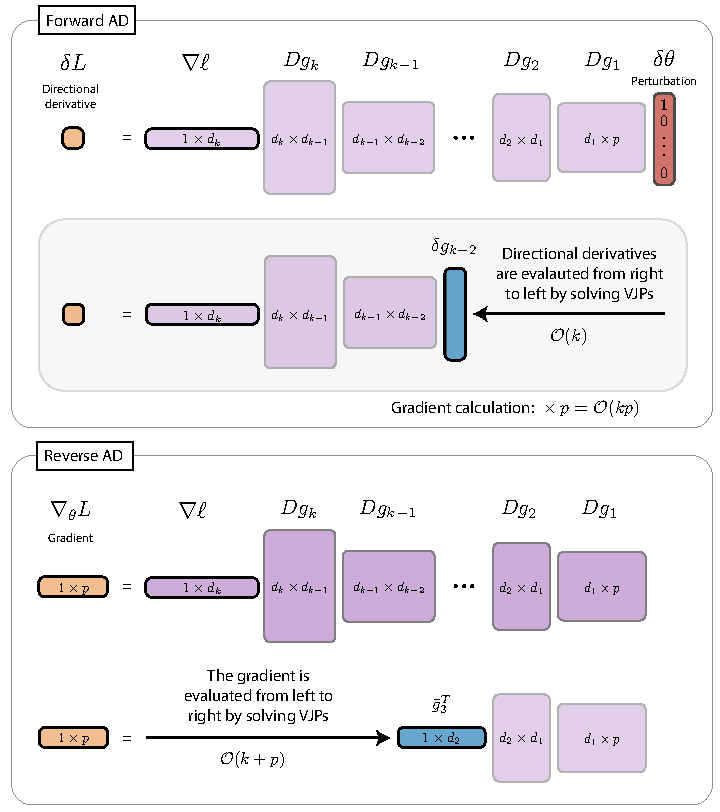
\includegraphics[width=0.85\textwidth]{figures/AD-VJPJVP.pdf}
    \caption{Comparison between forward and reverse mode AD. Changing the order of Jacobian and vector multiplications changes the total number of floating-point operations, which leads to different computational complexities between forward and reverse mode. When computing directional derivatives with forward AD, there is a total of $\mathcal O (k)$ JVPs that need to be computed, which considering we need to repeat this procedure $p$ times gives a total complexity of $\mathcal O (kp)$. This is the opposite of what happens when we carry the VJPs from the left side of the expression, where the matrix of size $d_1 \times p$ has no effect in the intermediate calculations, making all the intermediate calculations $\mathcal O (1)$ with respect to $p$ and a total complexity of $\mathcal O (k + p)$. }
    % However, backwards mode requires storing in memory information about the forward execution of the program, while forward mode can update the gradient on running time.}
    \label{fig:vjp-jvp}
\end{figure}

In practice, most AD systems are reduced to the computation of only directional derivatives (JVPs) or gradients (VJPs) \cite{Griewank:2008kh}.
Full Jacobians $J \in \R^{n \times p}$ (e.g., the sensitivity $s = \frac{\partial u}{\partial \theta} \in \R^{n \times p}$) can be fully reconstructed by the independent computation of the $p$ columns of $J$ via the JVPs $J e_i$, with $e_i \in \R^p$ the canonical vectors; or by the calculation of the $m$ rows of $J$ via the VJPs $e_j^T J$, with $e_j \in \R^n$.

% Sparsiity
% Sparse Jacobians are commonplace in large-scale nonlinear systems and discretized PDEs. 
% When the sparsity pattern is known, they can be efficiently obtained with colored AD to chunk multiple JVPs or VJPs, based on the colored Jacobian~\cite{gebremedhin2005color}.
% More concretely, consider the example of a Jacobian with known sparsity pattern given by
% \begin{equation}
%     {J}_{\text{sparse}} = \begin{bmatrix}
%         j_{11}  & 0       & 0       & 0       & 0       \\
%         0       & j_{22}  & j_{23}  & 0       & 0       \\
%         0       & 0       & 0       & j_{34}  & 0       \\
%         j_{41}  & j_{42}  & 0       & 0       & j_{45}  \\
%         0       & 0       & 0       & 0       & j_{55}
%     \end{bmatrix}.
% \end{equation}
% Computation of the non-zero entries $j_{ij}$ of the matrix ${J}_{\text{sparse}}$ can be performed by using AD for designed choices of vectors involved in the VJPs/JVPs \cite{pal2024nonlinearsolve}.
% Specifically, consider the following clustering of the $j_{ij}$'s indicated by different colors:   
% \begin{equation}
%     {J}^{(\text{col})}_{\text{sparse}} = 
%     \begin{bmatrix}
% \color{myred}{j_{11}} & 0 & 0 & 0 & 0\\
% 0 & \color{myblue}{j_{22}} & \color{myred}{j_{23}} & 0 & 0 \\
% 0 & 0 & 0 & \color{myred}{j_{34}} & 0 \\
% \color{myred}{j_{41}} & \color{myblue}{j_{42}} & 0 & 0 & \color{myviolet}{j_{45}} \\
% 0 & 0 & 0 & 0 & \color{myviolet}{j_{55}}
%     \end{bmatrix} 
%     \qquad 
%     {J}^{(\text{row})}_{\text{sparse}} = 
%     \begin{bmatrix}
% \color{myblue}{j_{11}} & 0 & 0 & 0 & 0 \\
% 0 & \color{myblue}{j_{22}}  & \color{myblue}{j_{23}} & 0 & 0 \\
% 0 & 0 & 0 &\color{myblue}{j_{34}} & 0 \\
% \color{myviolet}{j_{41}} & \color{myviolet}{j_{42}} & 0 & 0 & \color{myviolet}{j_{45}} \\
% 0 & 0 & 0 & 0 & \color{myblue}{j_{55}}
%     \end{bmatrix}.
% \end{equation}
% In the case of forward AD, we can compute three VJPs given by 
% \begin{equation}
%     J^{(\text{col})}_{\text{sparse}} 
%     \begin{bmatrix}
%     1 \\ 0 \\ 1 \\ 1 \\ 0    
%     \end{bmatrix}
%     = 
%     \begin{bmatrix}
%     \color{myred}{j_{11}} \\ \color{myred}{j_{23}} \\ \color{myred}{j_{34}} \\ \color{myred}{j_{41}} \\ 0 \\   
%     \end{bmatrix}, \qquad
%     J^{(\text{col})}_{\text{sparse}} 
%     \begin{bmatrix}
%     0 \\ 1 \\ 0 \\ 0 \\ 0    
%     \end{bmatrix}
%     = 
%     \begin{bmatrix}
%     0 \\ \color{myblue}{j_{22}} \\ 0 \\ \color{myblue}{j_{42}} \\ 0 \\
%     \end{bmatrix}, \qquad
%     J^{(\text{col})}_{\text{sparse}} 
%     \begin{bmatrix}
%     0 \\ 0 \\ 0 \\ 0 \\ 1    
%     \end{bmatrix}
%     = 
%     \begin{bmatrix}
%     0 \\ 0 \\ 0 \\ \color{myviolet}{j_{45}} \\ \color{myviolet}{j_{55}} \\ 
%     \end{bmatrix},
% \end{equation}
% while when using reverse AD we can instead compute two VJPs
% \begin{align}
% \begin{split}
%     \begin{bmatrix}
%     1 & 1 & 1 & 0 & 1    
%     \end{bmatrix}
%     \,
%     J^{(\text{row})}_{\text{sparse}} 
%     &= 
%     \begin{bmatrix}
%     \color{myblue}{j_{11}} & \color{myblue}{j_{22}} & \color{myblue}{j_{23}} & \color{myblue}{j_{34}} &    \color{myblue}{j_{55}}
%     \end{bmatrix} \\
%     \begin{bmatrix}
%     0 & 0 & 0 & 1 & 0    
%     \end{bmatrix}
%     \,
%     J^{(\text{row})}_{\text{sparse}} 
%     &= 
%     \begin{bmatrix}
%     \color{myviolet}{j_{41}} & \color{myviolet}{j_{42}} & 0 & 0 & \color{myviolet}{j_{45}}
%     \end{bmatrix}.\\
% \end{split}
% \end{align}
% In both cases, the full Jacobian ${J}_{\text{sparse}}$ is fully computed using a number of evaluations of VJPs/JVPs less than the five required to compute all entries of a dense Jacobian. 